\documentclass{beamer}
\usetheme{Madrid}
\usepackage{lmodern}% http://ctan.org/pkg/lm
\setbeamersize{text margin left = 2.5em}
\setbeamersize{text margin right = 2.5em}
\usepackage{color}
\usepackage{graphicx}
\usepackage{MnSymbol}
\usepackage{amsmath}
\usepackage{comment}
\usepackage{tikz}
\usepackage{subfigure}
\usepackage{listings}
\usetikzlibrary{automata}

%\usepackage[backend=bibtex,sorting=none]{biblatex}
%\addbibresource{E:/Papers/LiuLab} %BibTeX�����ļ���λ��
%\setbeamerfont{footnote}{size=\tiny}
\setbeamertemplate{theorems}[numbered]
\setbeamertemplate{caption}[numbered]
%% ʹ�ý�ע���õ�Ƭijҳ���Ӳο����ס�
%% ��������ʹ�ã�\footfullcite{bib_item} %����item
%% \usepackage{anyfontsize}%% allowing font sizes at arbitrary sizes
\logo{
\includegraphics[height=0.05\textwidth]{Pic/logo}}
\newtheorem{df}{Definition}
\newtheorem{DF}{DEFINITION}
\newtheorem{prop}{Proposition}
\newtheorem{thm}{Theorem}
\newtheorem{cor}{COROLLARY}
\newtheorem{lm}{LEMMA}
% ----------------------------------------------------------------------------------------
% TITLE PAGE
% ----------------------------------------------------------------------------------------

\title{E12 Backpropagation}
% The short title appears at the bottom of every slide, the full title is only on the title page

\author{Suixin Ou} % Your name
\institute[SYSU] % Your institution as it will appear on the bottom of every slide, may be shorthand to save space
{
  School of Computer Science\\
  Sun Yat-sen University \\ % Your institution for the title page
  \medskip
  % Your email address
}

\date{December 28, 2021} % Date, can be changed to a custom date

\AtBeginSection[]
{
  \begin{frame}
    \tableofcontents[currentsection,currentsubsection]
  \end{frame}
}

\begin{document}

\begin{frame}
  \titlepage
\end{frame}

\begin{frame}
  \frametitle{Background}
  \begin{block}{The Horse Colic Dataset}
    \begin{itemize}
    \item 
The UCI dataset (\url{http://archive.ics.uci.edu/ml/index.php}) is the most widely used dataset for machine learning. If you are interested in other datasets in other areas, you can refer to \url{https://www.zhihu.com/question/63383992/answer/222718972}.

    \item Colic in horses is defined as abdominal pain, but it is a clinical symptom rather than a diagnosis. Colic surgery is usually an expensive procedure as it is major abdominal surgery, often with intensive aftercare. Among domesticated horses, colic is the leading cause of premature death. So we want to predict whether a horse with colic will live or die in the Horse Colic Dataset.

    \end{itemize}
      
  \end{block}
\end{frame}


\begin{frame}
  \frametitle{Task}
  \begin{block}{Description}
	
    \begin{itemize}
      \item Dataset statistics

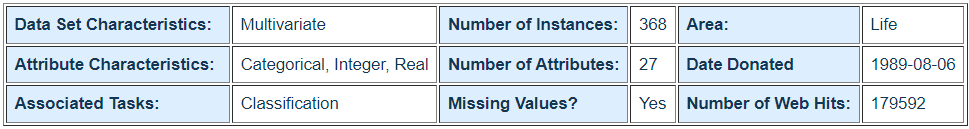
\includegraphics[width=0.85\textwidth]{Pic/dataset}
      \item Domain information

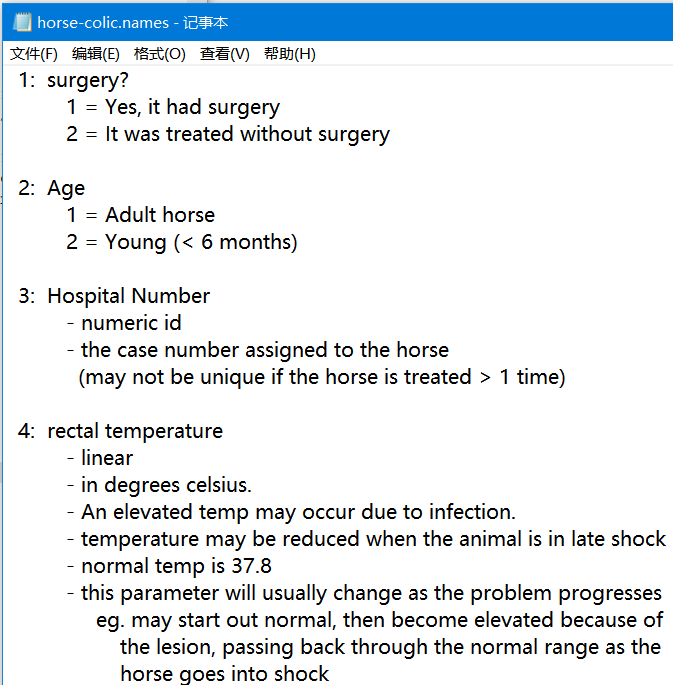
\includegraphics[width=0.35\textwidth]{Pic/domain}
% 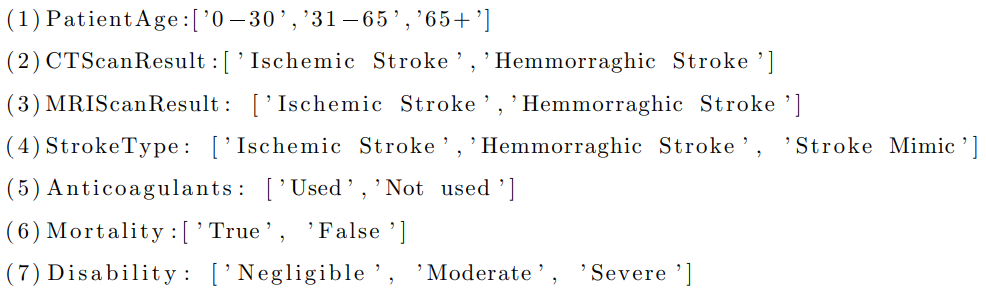
\includegraphics[width=10cm]{Pic/e21}
% 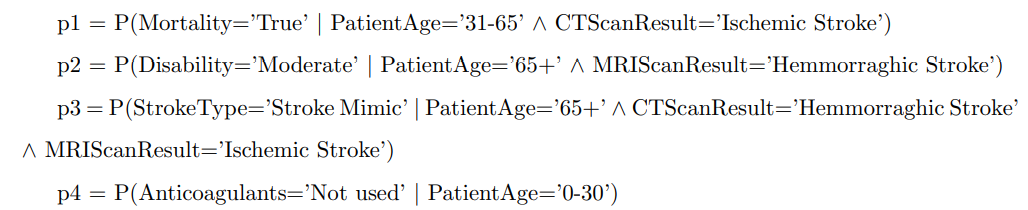
\includegraphics[width=10cm]{Pic/e22}
    \end{itemize}

  \end{block}
\end{frame}


\begin{frame}
  \frametitle{Solution}
      Read the file "horse-colic.data" or "horse-colic.test"
      \\[10pt]
      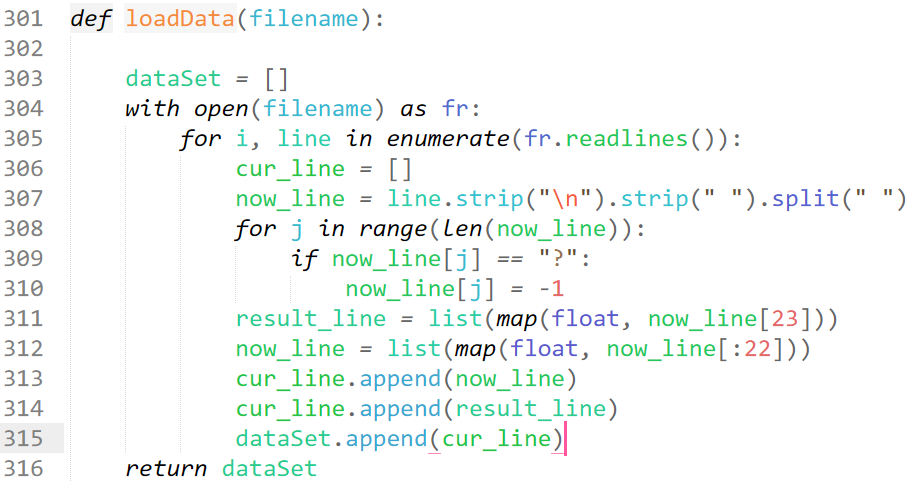
\includegraphics[width=1.0\textwidth]{Pic/loadData.png}


\end{frame}

\begin{frame}
  \frametitle{Solution}

      Initialize parameters
      \\[10pt]
      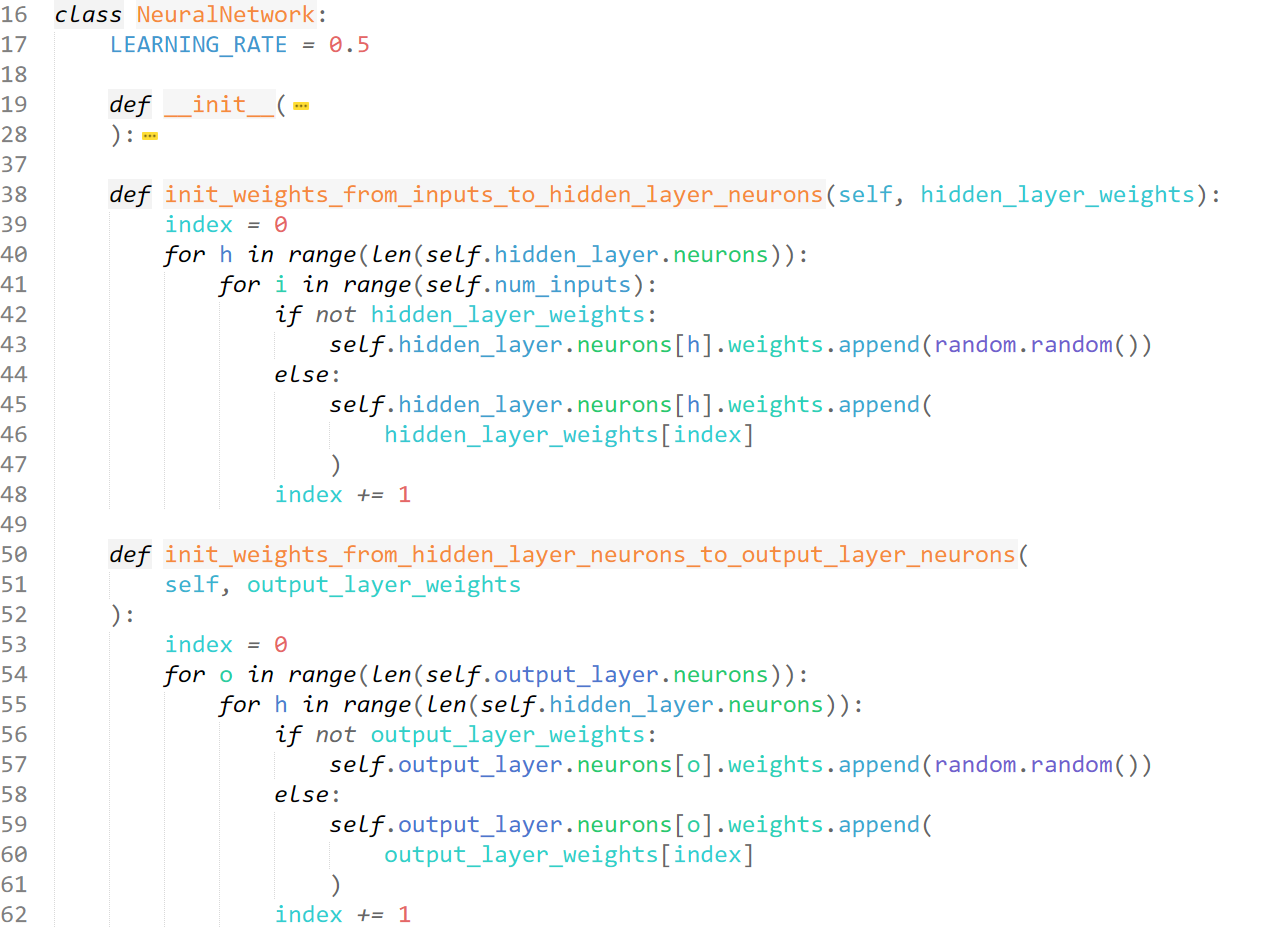
\includegraphics[width=1.0\textwidth]{Pic/init_params.png}

\end{frame}

\begin{frame}
  \frametitle{Solution}
	   Visualization
      \\[10pt]
      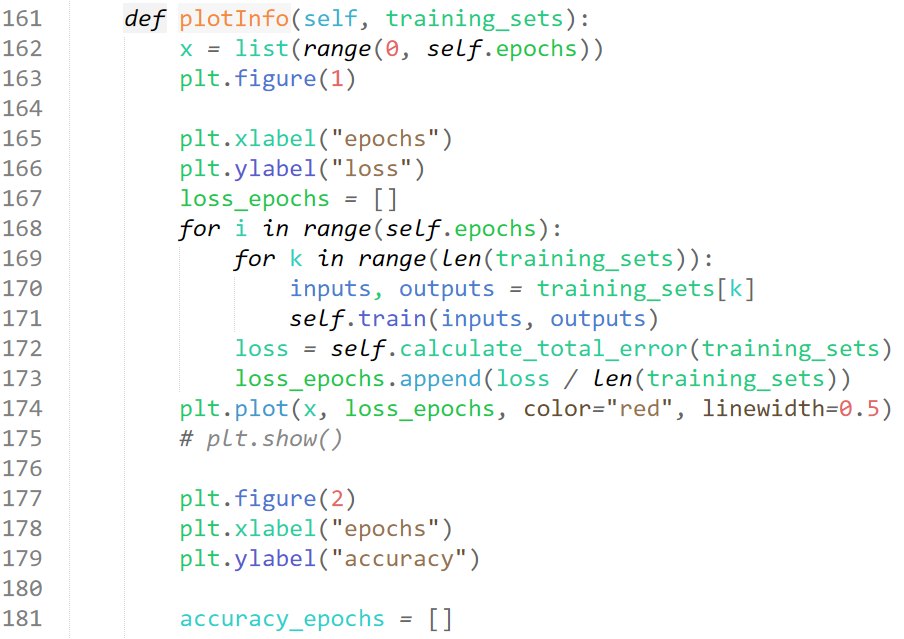
\includegraphics[width=1.0\textwidth]{Pic/visualization.png}

\end{frame}

\begin{frame}
  \frametitle{Solution}
	   Training, testing and visualization framework
      \\[10pt]
      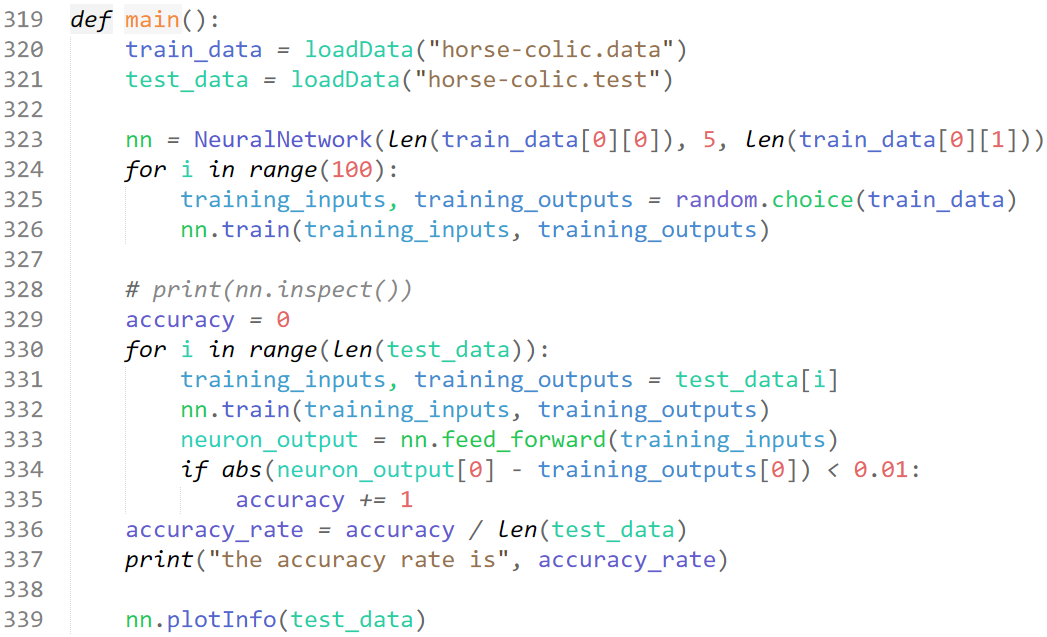
\includegraphics[width=1.0\textwidth]{Pic/framwork.png}

\end{frame}

\begin{frame}
  \frametitle{Solution}
	  Forward calculation.
      \\[10pt]
      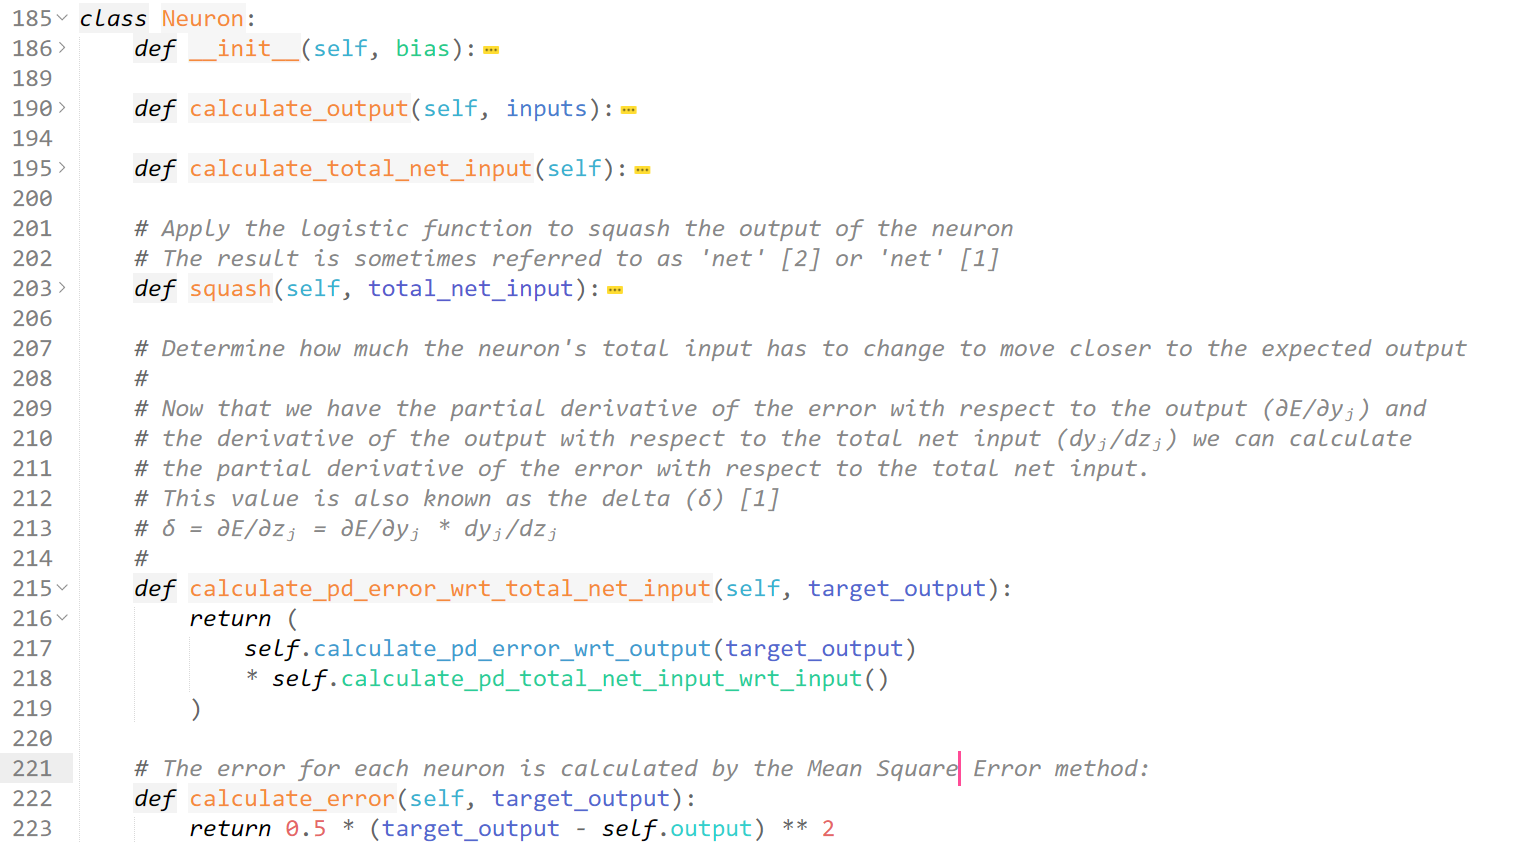
\includegraphics[width=0.9\textwidth]{Pic/forward.png}

\end{frame}

\begin{frame}
  \frametitle{Solution}
	  \textbf{Please Finish the Backward Propagation.}
      \\[10pt]
      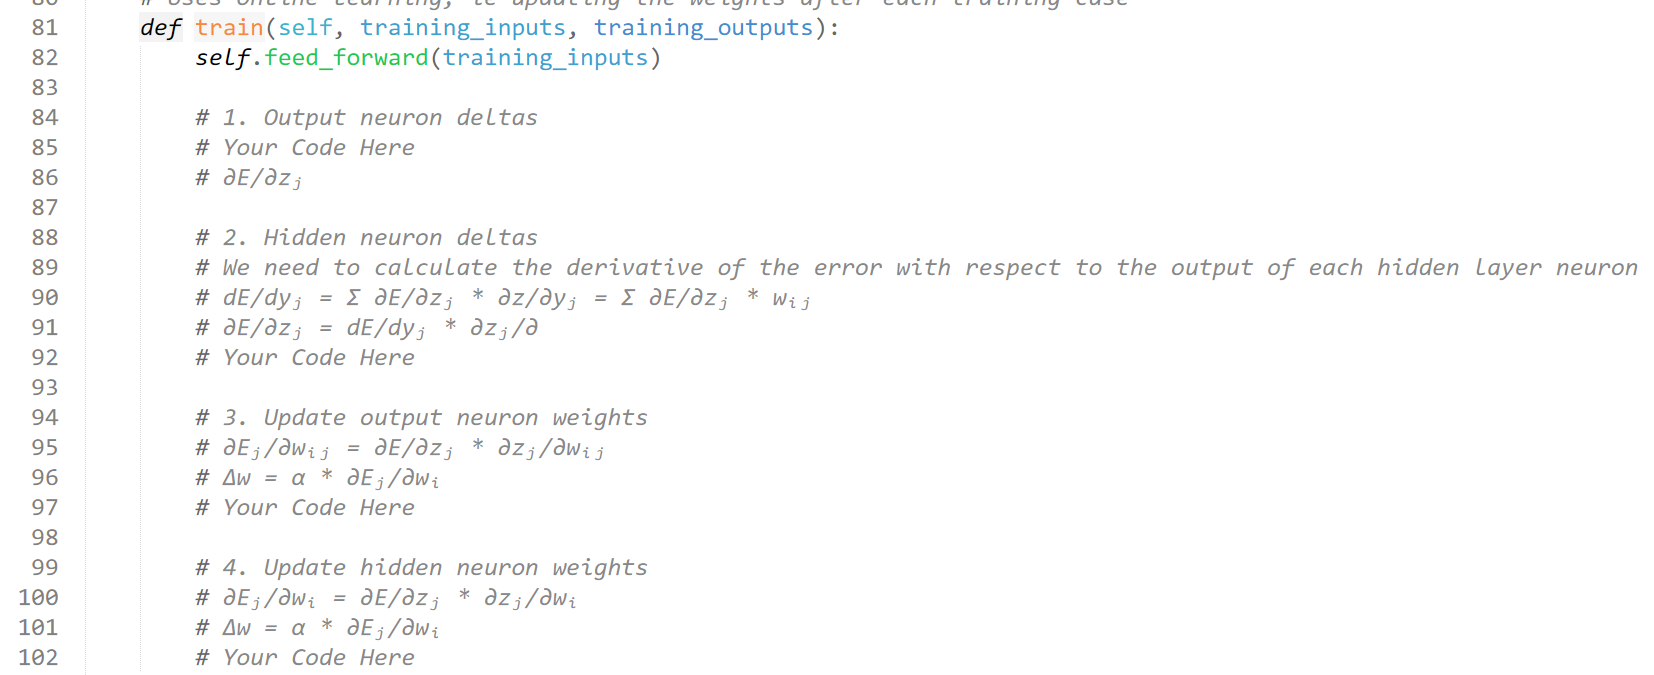
\includegraphics[width=0.9\textwidth]{Pic/bp.png}

\end{frame}


\begin{frame}
  \frametitle{Submission}
  \begin{block}{Submission}
    pack your report \texttt{E12\_YourNumber.pdf} and source code into zip file \texttt{E12\_YourNumber.zip}, then send it to \texttt{ai\_course2021@163.com}.
  \end{block}
\end{frame}

\begin{frame}
  \frametitle{Optional exercise: Deep Learning}
  \begin{block}{Convolutional Network and Cifar-10 Dataset}
    \begin{itemize}
    \item 
    So far we have worked with deep fully-connected networks and backward propagation. Fully-connected networks are a good testbed for experimentation because they are very computationally efficient, but in practice state-of-the-art results in Cifar-10 Dataset use convolutional networks instead.
    \item 
You can implement several layer types that are used in convolutional networks, then use these layers to train a convolutional network on the CIFAR-10 dataset.
    \item The CIFAR-10 dataset consists of 60000 32x32 colour images in 10 classes, with 6000 images per class. There are 50000 training images and 10000 test images. The target is to predict the class for unseen examples.\\
    \item I suggest you to refer to https://github.com/maxis42/CS231n/blob/master/assignment2/ConvolutionalNetworks\_2018.ipynb.
    \end{itemize}

  \end{block}
\end{frame}

%-----------------------------------------------------------------------------------------

\begin{frame}
  \Huge{\centerline{The End}}
\end{frame}

% ----------------------------------------------------------------------------------------


\end{document}
